\documentclass[final]{article}
\usepackage{bm}
\usepackage{amsmath}
\usepackage{amssymb}
\usepackage{hyperref}
\usepackage{rotating}
\usepackage{float}
\usepackage{graphicx}
\usepackage{wrapfig}
\usepackage{subcaption}
\usepackage{amsmath, mathtools}
\usepackage{listings}
\usepackage{color}
\usepackage[extrafootnotefeatures, Kashida]{xepersian}
\usepackage{multirow}
\usepackage{fourier}
\settextfont{XB Niloofar}
\setdigitfont{XB Niloofar}
\hypersetup{
	colorlinks=true,
	linkcolor=blue,
	filecolor=blue,      
	urlcolor=cyan,
}
\definecolor{dkgreen}{rgb}{0,0.6,0}
\definecolor{gray}{rgb}{0.5,0.5,0.5}
\definecolor{mauve}{rgb}{0.58,0,0.82}
\definecolor{apricot}{rgb}{0.98046, 0.894,0.8014}
\lstset{ %
	language=R,                     % the language of the code
	basicstyle=\footnotesize,       % the size of the fonts that are used for the code
	numbers=left,                   % where to put the line-numbers
	numberstyle=\tiny\color{gray},  % the style that is used for the line-numbers
	stepnumber=1,                   % the step between two line-numbers. If it's 1, each line
	% will be numbered
	numbersep=5pt,                  % how far the line-numbers are from the code
	backgroundcolor=\color{apricot},  % choose the background color. You must add \usepackage{color}
	showspaces=false,               % show spaces adding particular underscores
	showstringspaces=false,         % underline spaces within strings
	showtabs=false,                 % show tabs within strings adding particular underscores
	frame=single,                   % adds a frame around the code
	rulecolor=\color{black},        % if not set, the frame-color may be changed on line-breaks within not-black text (e.g. commens (green here))
	tabsize=2,                      % sets default tabsize to 2 spaces
	captionpos=b,                   % sets the caption-position to bottom
	breaklines=true,                % sets automatic line breaking
	breakatwhitespace=false,        % sets if automatic breaks should only happen at whitespace
	title=\lstname,                 % show the filename of files included with \lstinputlisting;
	% also try caption instead of title
	keywordstyle=\color{blue},      % keyword style
	commentstyle=\color{dkgreen},   % comment style
	stringstyle=\color{dkgreen},      % string literal style
	escapeinside={\%*}{*)},         % if you want to add a comment within your code
	morekeywords={*,...}            % if you want to add more keywords to the set
} 
\def\ojoin{\setbox0=\hbox{$\bowtie$}%
	\rule[-.02ex]{.25em}{.4pt}\llap{\rule[\ht0]{.25em}{.4pt}}}
\def\leftouterjoin{\mathbin{\ojoin\mkern-5.8mu\bowtie}}
\def\rightouterjoin{\mathbin{\bowtie\mkern-5.8mu\ojoin}}
\def\fullouterjoin{\mathbin{\ojoin\mkern-5.8mu\bowtie\mkern-5.8mu\ojoin}}


%\makeatletter
%\renewcommand{\thesection}{%
%  \ifnum\c@chapter<1 \@arabic\c@section
%  \else \thechapter.\@arabic\c@section
%  \fi
%}
%\makeatother

\title{
طراحی سیستم‌های دیجیتال
	\\
	{
		\large
		گزارش نهایی پروژه‌ی سوم
	}
}
\author{
	\begin{tabular}{rl}
		مهبد مجید	&
		۹۵۱۰۹۳۷۲
		\\
		سبحان محمدپور & 
		۹۵۱۰۶۶۰۷
		\\
		کیمیا حمیدیه &
		۹۵۱۰۹434
		\\
		روژین نوبهاری
		&
		۹۵۱۰۵۲۳۸
		\\
		کوشا جافریان
		&
		۹۵۱۰۵۴۵۴
	\end{tabular}
}

\begin{document}
	\maketitle
	
	\section*{توصیف اولیه}
\subsection*{مقدمه}
امروزه با توجه به کاربرد گسترده‌ی
\lr{Java}
و بالطبع
\lr{JVM}
،
در صنعت و جهان مدرن امروزی منطقی به نظر می‌رسد که فرآیند اجرای کدهای جاوا را سریع‌تر کنیم.
یکی از راه‌های خوب برای رسیدن به این مهم، می‌تواند پیاده‌سازی سخت‌افزاری 
\lr{JVM}
که در واقع هسته‌ی جاواست  باشد.
\subsection*{اهداف}
در این پروژه می‌خواهیم برای پردازنده‌ی 
\lr{ARM-7}(صبای ۲)
یک شتاب‌دهنده‌
\LTRfootnote{accelerator}
‌ی سخت‌افزاری
\lr{JVM}
بسازیم.
نحوه‌ی کار این شتاب‌دهنده به این شکل است که پردازنده 
\lr{opcode}های
\lr{JVM}
را دریافت می‌کند و به شتاب‌دهنده می‌دهد و شتاب‌دهنده دستورات معادل پردازنده را تولید می‌کند.
\subsection*{مراحل انجام پروژه}
به طور کلی با توجه به اهداف پروژه ما باید ۳ کار را برای انجام پروژه انجام‌دهیم:
\begin{itemize}
	\item 
	یادگیری کار با ماشین
	\lr{JVM}
	\item
	یادگیری کار با ماشین
	\lr{ARM-7}
	\item
	ساخت مبدل برای تبدیل دستورات میان این دو
\end{itemize}
	
	\section*{تقسیم‌بندی پروژه}
\subsection*{انتخاب
	\lr{opcode}ها}
ابتدا لیست
\lr{opcode}های
\lr{JVM}
را پیداکردیم. از آنجایی که قرار بود این پروژه برای ۵ تیم باشد، نیاز بود تا تعدادی از آپکدها را جداکنیم که پروژه برای ۴ تیم مناسب شود.
برای جداکردن تعدادی از این
\lr{opcode}ها
از
\lr{Jazelle}
الگو می‌گیریم. 
\lr{Jazelle}
به این صورت عمل می‌کند که
\lr{JVM}
دستوراتش را به
\lr{Jazelle}
می‌فرستد و اگر
\lr{Jazelle}
از آن‌ها پشتیبانی کرد، آن‌ها را اجرا می‌کند، و اگر هم پشتیبانی نمی‌کرد آن‌ها را به
\lr{JVM}
باز می‌گرداند تا آن‌ها را به دستوراتی که
\lr{Jazelle}
از آن‌ها پشتیبانی می‌کند تبدیل کند.
\begin{figure}[H]
	\centering
	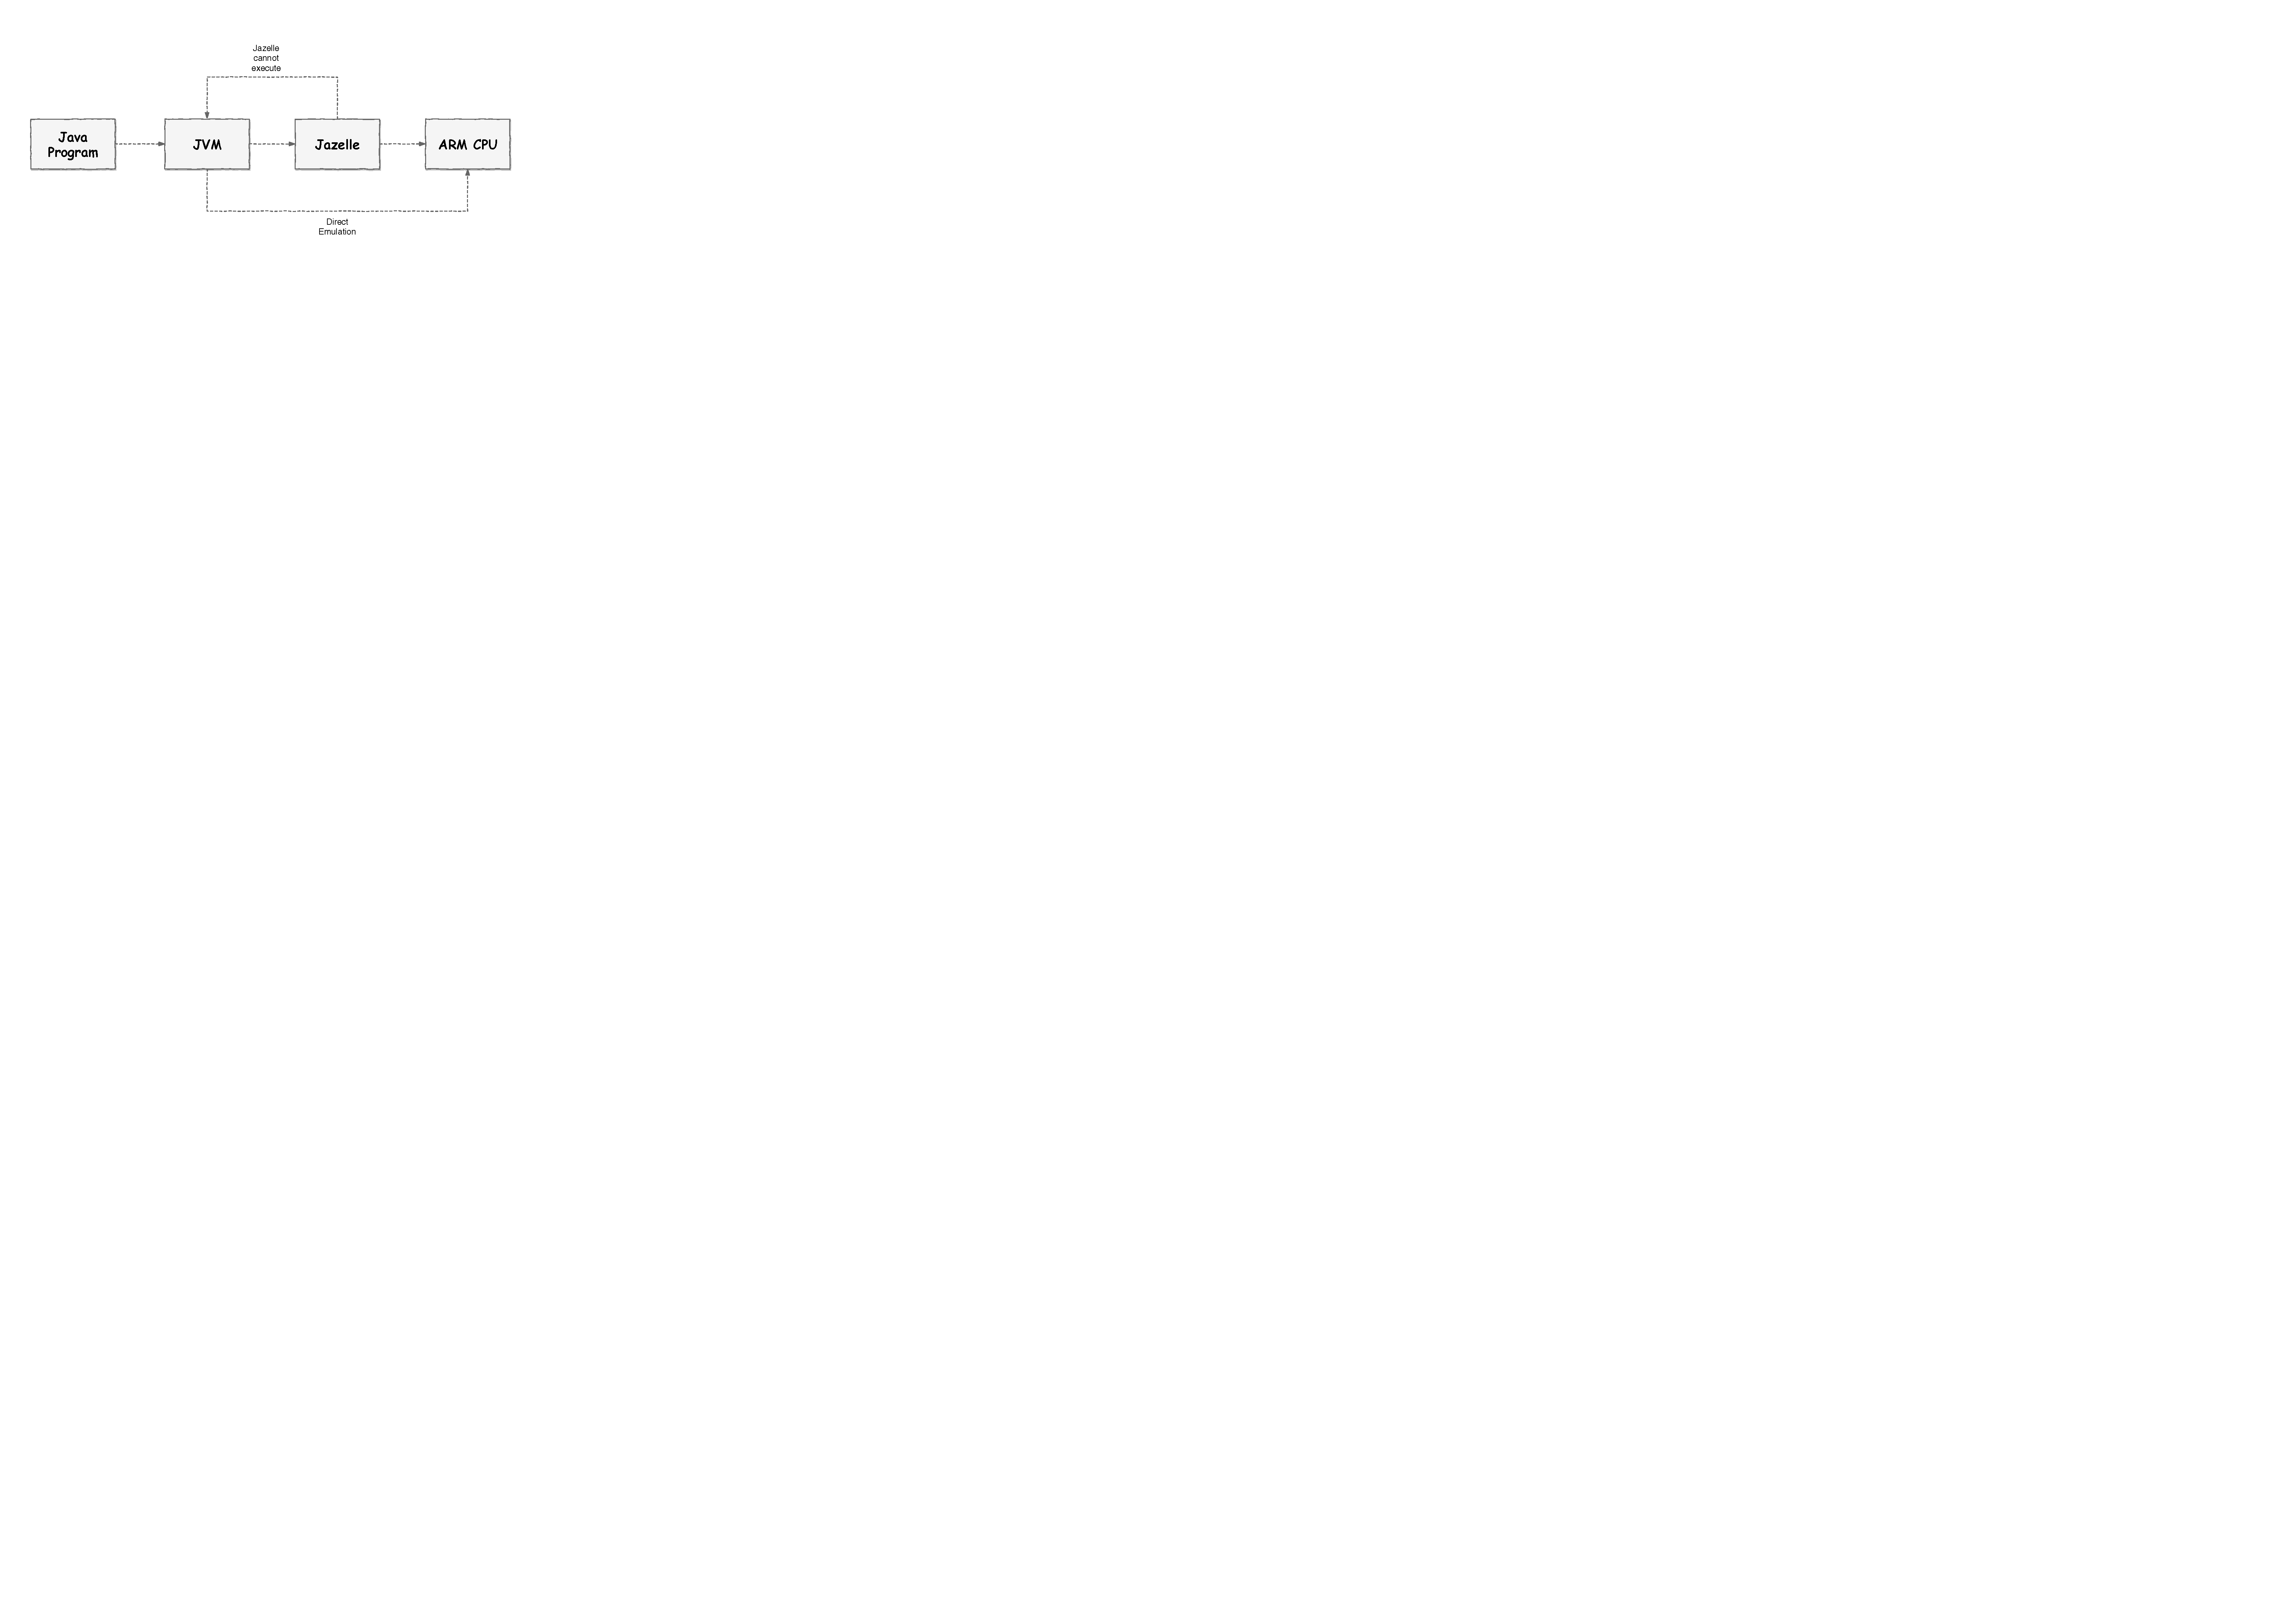
\includegraphics[width=\linewidth]{flowchart}
	\caption{روند اجرای کار jazelle}
	\label{fig:flowchart}
\end{figure}

ما نیز به این صورت عمل می‌کنیم که عده‌ای از 
\lr{opcode}ها
که پیاده‌سازی نرم‌افزاریشان ساده‌تر است را جدا می‌کنیم و الباقی
\lr{opcode}ها 
را در پیاده‌سازیمان می‌آوریم.
\subsection*{تقسیم‌بندی 
	\lr{opcode}ها
}
برای افزایش بازدهی گروه‌ها
\lr{opcode}های
انتخابی به شانزده بسته‌ی ۱۰تایی تقسیم‌بندی شدند و با یک کد 
\lr{R}
که به صورت رندوم این ۱۶ بسته را به گروه‌ها تخصیص می‌داد، تقسیم‌بندی کردیم.(سید را هم با حضور اعضای سایر گروه‌ها تعیین‌کردیم.)
\subsubsection*{کد}
\begin{latin}
	\begin{lstlisting}
	library(dplyr)
	set.seed(1919)
	s = sample(seq(from = 1, to = 16), replace = F)  
	c("jaferian", "asadi", "hoseini", "ghafarloo") %>% 
	cbind(t(apply(matrix(s, nrow = 4), 1, sort)))
	\end{lstlisting}
\end{latin}
\subsubsection*{خروجی کد}
\begin{latin}
	\centering
	\begin{tabular}{l|cccc}
		Group Name & & & & \\
		\hline \hline
		jaferian & 4 & 6 & 7 & 8\\
		
		asadi & 3 & 9 & 10 & 12\\
		hoseini & 1 & 5 & 11 & 14\\
		ghafarloo & 2 & 13 & 15 & 16\\
	\end{tabular}
\end{latin}
\subsubsection*{لیست دستورات}
لیست دستورات را می‌توانید در صفحه‌گسترده‌ی ۱ و ۲ مشاهده‌کنید.


	\section*{
	برخی ]dماژول‌های پیاده‌سازی‌شده با
	\lr{verilog}
}

\subsection*{فایل 
	\lr{memory.v}
}
در این فایل دو ماژول حافظه طراحی شده‌است. ماژول اول
\lr{memory\_r}
است که به عنوان ورودی سیگنال‌های کلاک
\LTRfootnote{clk}
، ریست
\LTRfootnote{reset}
، شروع
\LTRfootnote{start}
و آدرس
\LTRfootnote{address}
را می‌گیرد. در ضمن دو سیگنال خروجی داده‌ی مورد نظر
\LTRfootnote{data\_out}
و آماده‌بودن رم و جواب
\LTRfootnote{ready}
را هم داریم. حال در این ماژول، با فعال‌شدن سیگنال شروع، منتظر می‌مانیم تا سینگال 
\lr{ready}
حافظه فعال شود.
در اصل وجود
\lr{start}
و 
\lr{ready}
به شکل پیاده‌سازی‌شده برای پیاده‌سازی تاخیر حافظه بوده‌است.
به محض فعال‌شدن
\lr{ready}،
از آدرس مورد نظر، محتوا را خوانده و در 
\lr{data\_out}
خروجی می
دهیم.
ماژول دوم نیز
\lr{memory\_w}
است که برای نوشتن در حافظه استفاده می‌شود.
توجه‌کنید که در این جا دیگر لازم نیست
\lr{data\_out}
را خروجی‌دهیم و تنها هنگام
فعال‌شدنِ
\lr{start}
در حالت نوشتن، صبر می‌کنیم تا سیگنال
\lr{ready}
حافظه فعال‌شود و به محض فعال‌شدن در
\lr{address}
مورد نظر محتوای مربوطه را می‌نویسیم. توجه‌کنید که تنها تفاوت اساسی با
\lr{memory\_r}
این است که به جای خروجی
\lr{data\_out}
یک ورودی
\lr{data\_in} 
داریم که محتوایی که باید در حافظه نوشته‌شود را مشخص می‌کند.
\subsection*{
	فایل
	\lr{next\_byte\_gen.v}
}
همان‌طور که می‌دانیم؛ در پردازنده‌هایِ واقعیِ
\lr{JVM}،
هنگام خواندن و نوشتن در حافظه، با بایت سر و کار نداریم؛ بلکه برای مثال موقع خواندن یک
\lr{word}ِ
4	 بایتی از حافظه خوانده می‌شود. در بسیاری از مواقع این
\lr{word}،
شامل چندین بایت است که برای دسترسی به مواردی مانند opcode یا offset باید این بایت‌ها را جداجدا بخوانیم. برای این منظور ماژول
\lr{next\_byte\_gen}
طراحی شده‌است که یک
\lr{memory\_r}
را instantiate کرده و در صورتی که هر دو سیگنال start و ready فعال باشند؛ PC که برابر
\lr{address}ِ
حافظه‌ی instantiate شده‌است را یک واحد اضافه می‌کند که معادل یک بایت جلورفتن یا رفتن به بایت بعدی است و در صورت فعال‌بودنِ reset نیز، مقداری پیش‌فرض را برابر PC قرار خواهد داد.
\subsection*{فایل
	\lr{instruction\_ram.v}}
این ماژول نیز کار پیچیده‌ای انجام نمی‌دهد و تنها یک
\lr{word}ِ
۴ بایتی را از ورودی دریافت‌کرده و درون یک حافظه‌ی نوشتنی
\lr{(memory\_w)}
می‌نویسد. برای این کار کافیست تا هنگام instantiate کردن این حافظه درون ماژول،
\lr{data\_in}ِ
آن را برابر 
\lr{word}ِ
خوانده‌شده از ورودی قراردهیم. بدیهی‌است که سایر پارامترها نیز باید به درستی تنظیم شوند.
\subsection*{فایل‌های مربوط به 
	\lr{Decoder}}


دیکُدر طراحی‌شده در این پروژه به صورت
چند ماژول
\lr{Read Only Memory( ROM)} 
طراحی شده‌است. این 
\lr{ROM}ها
عبارتند از: 
\subsubsection*{
	\lr{Address ROM}
}
این ROM یک آدرس به عنوان ورودی گرفته و آدرس
بعدی که پس از این آدرس باید به آن برویم را برمیگرداند. 
\subsubsection*{
	\lr{Convert ROM}
}
این ROM یک آدرس را به عنوان ورودی گرفته و به عنوان
خروجی ID دستور مربوطه را به ما تحویل می‌دهد. 
\subsubsection*{
	\lr{Instruction ROM}
}
این 
\lr{ROM}،
\lr{ID}ِ
دستور را گرفته و خود دستور را به ما می
دهد. منظور از خروجی‌دادن خود دستور، پیاده‌سازی آن به صورت 0 و 1 درون ROM  است. توجه‌کنید که برای پیاده‌سازی این ROM، ابتدا دستورات پردازنده را با زبان
اسمبلی ARM نوشتیم و سپس به کمک یک قطعه‌کد پایتون به صورت خودکار آن‌ها را به فرمت کدشده 0 و 1 که باید درون این ROM نوشته‌شود؛ در می‌آوریم.
\subsection*{توضیحی درباره توالی آٓدرس‌ها}
توجه‌کنید که هنگامی که یک دستور را می خوانیم؛ ابتدا در آدرس مربوط به Opcode آن دستور قرار داریم، اما پس از آن با موارد تعیین شده در 
\lr{Address ROM}،
به صورت زنجیره‌ای (مانند یک لیست پیوندی) جلورفته و به ترتیب مجموعه عملیات مشخصی را انجام خواهیم داد. (توجه‌کنید که ممکن است یک دستور JVM به چندین دستور ARM تبدیل شود بنابراین باید زنجیره‌ای از دستورات را به ترتیب اجرا کنیم!) توجه کنید که
\lr{Convert ROM}
نیز ورودی آدرس را گرفته و یک ID را تحویل 
\lr{Instruction ROM}
می‌دهد و این ROM وظیفه اجرای دستور را خواهد داشت.

\subsection*{
	فایل
	\lr{Count ROM}}
این ROM برای این پیاده‌سازی شده‌است که مشخص‌کند پس از
خواندن Opcode یک دستور، چند بایت آینده مربوط به ادامه این دستور خواهد بود. توجه‌کنید که برخی از دستورات ممکن است تنها از یک بایت که همان Opcode است تشکیل‌شده باشند مثلا Pop ولی بسیاری از دستورات هستند که مواردی مانند یک 
\lr{Offset}
2 بایتی یا مشابه آن دارند. بنابراین
\lr{Count ROM}
با گرفتن
Opcode مشخص
می‌کند که دستور مربوطه چند بایت اضافی دارد. توجه‌کنید که در فاز اول پروژه که شامل 
$40 \%$
کار می‌شود؛ مواردی که شامل حداکثر 2 بایت اضافه باشد را Handle کرده‌ایم و تمامی موارد در فاز نهایی پروژه پیاده‌سازی خواهند شد.
\begin{itemize}
	\item[
	\danger\textbf{توجه مهم}
	]
	همان‌طور که ذکر شد؛ دستورات ممکن است پس از 
	\lr{Opcode}
	تعدادی immediate داشته باشند که پارامترهایی مانند
	\lr{index}،
	\lr{varnum}
	یا offset را مشخص کنند. برای راحتی کار، در پیاده‌سازی خود، این پارامترها را درون یکی از ثبات‌های پردازنده ARM می‌ریزیم و به درون استک Push ، ARM می‌کنیم. این کار سبب می‌شود که دیگر نیازی به انجام تغییر در
	\lr{Instruction ROM}
	نباشد و عملا پیاده‌سازی ما به مراتب راحت‌تر خواهد شد.
\end{itemize}
	
	\section*{
ماشین حالت
\LTRfootnote{State Machine}
}
حالات ماشین حالت را می‌توانید در شکل زیر مشاهده نمایید:
\begin{figure}[H]
	\centering
	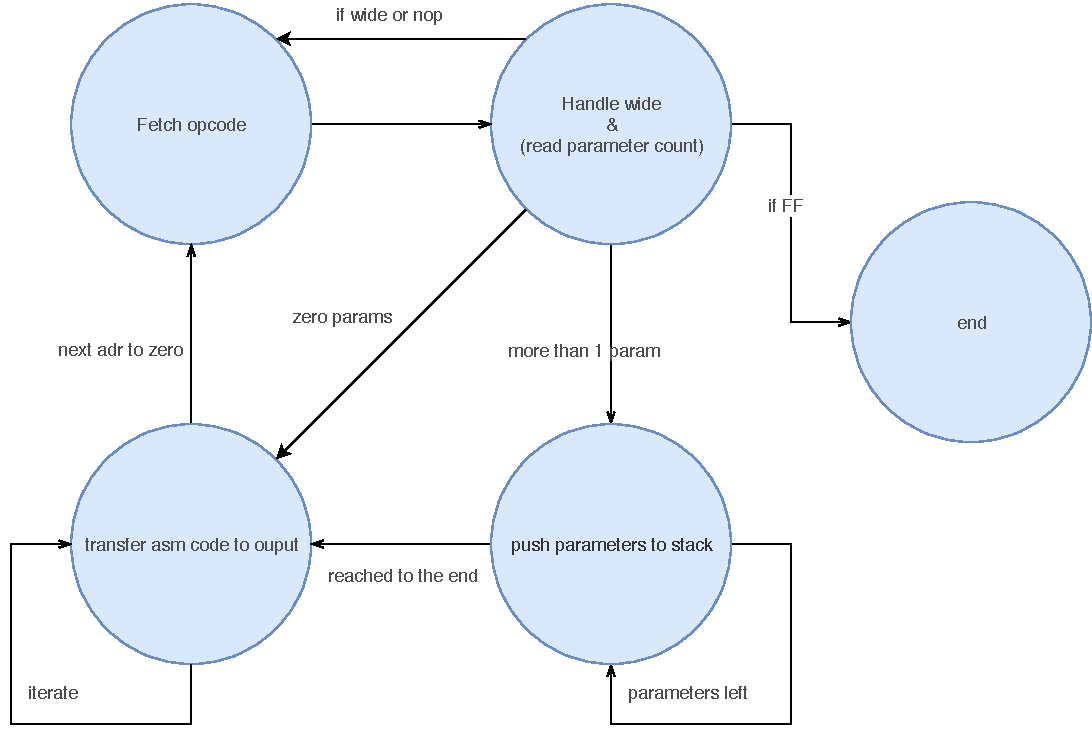
\includegraphics[width=0.9\linewidth]{SM}
	\caption{ماشین حالت}
	\label{fig:sm}
\end{figure}
%%% May add some information
\subsection*{\lr{FETCH\_INSTRUCTION}}
در این استیت، آپکد دستور 
\lr{JVM}،
 از رم مربوط به آن خوانده می‌شود. و بعد برای بررسی نوع دستور و گرفتن تعداد پارامترهای آن، به استیت (۲) می‌رویم. 

\subsection*{\lr{CHECK\_WIDE\_AND\_READ\_COUNTER}}

با بررسی آپکد دستور که در مرحله‌ی قبل خوانده‌ایم، در این‌جا با بررسی نوع دستور، به یکی از استیت‌های زیر می‌رویم:
\subsection*{\lr{END}}
برای پایان برنامه از یک بایت که در دستورات JVM نیست
\LTRfootnote{reserved word}
 مانند
\lr{0xFF}
استفاده کرده‌ایم. در صورتی که آپکد برابر این کلمه باشد، برنامه‌ی داخل رم JVM تمام شده‌است و کار این ماژول به پایان می‌رسد. 
\subsection*{ITERATE}
با استفاده از
\lr{count\_rom}
-که همان‌طور که قبلاً توضیح داده شده‌است، ماژولی است که با توجه به آپکد دستوراتِ
\lr{JVM}،
  تعداد بایت پارامترهایی که بعد از آن آپکد قرار می‌گیرند را مشخص می‌کند - می‌توان تعداد پارامترهای هر آپکد را در این‌جا داشت. بنابراین اگر پارامتری پس از این آپکد نداشته باشیم، مستقیماً به این استیت می‌رویم.
	
	\section*{مراجع}
\begin{itemize}
	\item
	داک JVM در سایت ORACLE موجود در 
	\begin{latin}
	\href{https://docs.oracle.com/javase/specs/jvms/se7/html/index.html}{JSR-000924 Java® Virtual Machine Specification}
	\end{latin}
\end{itemize}
\end{document} 